\documentclass[10pt]{beamer}
\usetheme[
%%% options passed to the outer theme
%    hidetitle,           % hide the (short) title in the sidebar
%    hideauthor,          % hide the (short) author in the sidebar
%    hideinstitute,       % hide the (short) institute in the bottom of the sidebar
%    shownavsym,          % show the navigation symbols
%    width=2cm,           % width of the sidebar (default is 2 cm)
%    hideothersubsections,% hide all subsections but the subsections in the current section
%    hideallsubsections,  % hide all subsections
%    left                % right of left position of sidebar (default is right)
  ]{Aalborg}
  
% If you want to change the colors of the various elements in the theme, edit and uncomment the following lines
% Change the bar and sidebar colors:
%\setbeamercolor{Aalborg}{fg=red!20,bg=red}
%\setbeamercolor{sidebar}{bg=red!20}
% Change the color of the structural elements:
%\setbeamercolor{structure}{fg=red}
% Change the frame title text color:
%\setbeamercolor{frametitle}{fg=blue}
% Change the normal text color background:
%\setbeamercolor{normal text}{bg=gray!10}
% ... and you can of course change a lot more - see the beamer user manual.

\usepackage[utf8]{inputenc}
\usepackage[english]{babel}
\usepackage[T1]{fontenc}
% Or whatever. Note that the encoding and the font should match. If T1
% does not look nice, try deleting the line with the fontenc.
\usepackage{helvet}


% colored hyperlinks
\newcommand{\chref}[2]{%
  \href{#1}{{\usebeamercolor[bg]{Aalborg}#2}}%
}

\title[Semantic Web Mining]% optional, use only with long paper titles
{Semantic Web Mining}

\subtitle{Semantic Web Course}  % could also be a conference name

\date{\today}

\author[Ali Mohebbi, Mehdi Keshani] 
 % optional, use only with lots of authors
{
  Ali Mohebbi\\
  \href{mailto:a.mohebbi@ce.sharif.edu}{{\tt a.mohebbi@ce.sharif.edu}}\\
   Mehdi Keshani\\
  \href{mailto:keshani@ce.sharif.edu}{{\tt keshani@ce.sharif.edu}}
}

% - Give the names in the same order as they appear in the paper.
% - Use the \inst{?} command only if the authors have different
%   affiliation. See the beamer manual for an example

\institute[
%  {\includegraphics[scale=0.2]{aau_segl}}\\ %insert a company, department or university logo
  Dept.\ of Computer Engineering\\
  Sharif University\\
  Iran
] % optional - is placed in the bottom of the sidebar on every slide
{% is placed on the bottom of the title page
  Dept.\ of Computer Engineering\\
  Sharif University\\
  Iran
  
  %there must be an empty line above this line - otherwise some unwanted space is added between the university and the country (I do not know why;( )
}

% specify the logo in the top right/left of the slide
\pgfdeclareimage[height=1cm]{mainlogo}{AAUgraphics/aau_logo_new} % placed in the upper left/right corner
\logo{\pgfuseimage{mainlogo}}

% specify a logo on the titlepage (you can specify additional logos an include them in 
% institute command below
\pgfdeclareimage[height=1.5cm]{titlepagelogo}{AAUgraphics/aau_logo_new} % placed on the title page
%\pgfdeclareimage[height=1.5cm]{titlepagelogo2}{AAUgraphics/aau_logo_new} % placed on the title page
\titlegraphic{% is placed on the bottom of the title page
  \pgfuseimage{titlepagelogo}
%  \hspace{1cm}\pgfuseimage{titlepagelogo2}
}
\usepackage{ragged2e}
\usepackage{etoolbox}
\usepackage{lipsum}
\usepackage{subcaption}
\usepackage{mathtools}
\apptocmd{\frame}{}{\justifying}{}
\begin{document}
% the titlepage
{\aauwavesbg
\begin{frame}[plain,noframenumbering] % the plain option removes the sidebar and header from the title page
  \titlepage
\end{frame}}
%%%%%%%%%%%%%%%%

% TOC
\begin{frame}{Agenda}{}
\tableofcontents
\end{frame}
%%%%%%%%%%%%%%%%


\section{Data Mining}
\begin{frame}{Data Mining}

\begin{itemize}
\item Data mining is the study of collecting, cleaning, processing, analyzing, and gaining useful
insight from data  \cite{han2011data}.
\item Data mining is a broad term that is used to describe different aspects of data processing
(depending on the problem domain, applications, formulation, and data representations).

\end{itemize}
\begin{figure}[H]
	\centering
	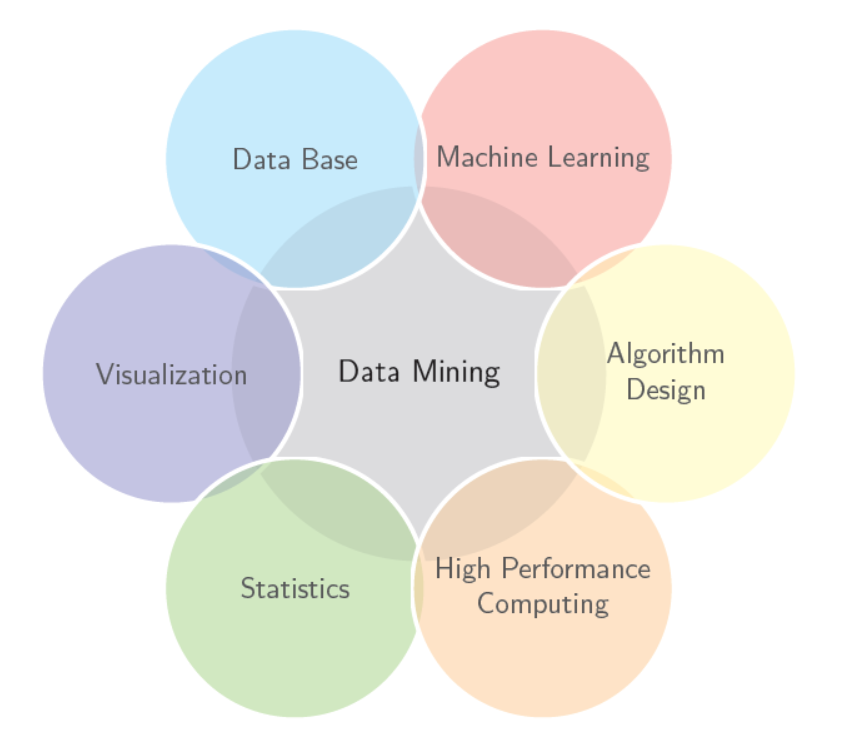
\includegraphics[width=0.4\textwidth]{images/DataMining.PNG}
	\label{fig:DataMining}
\end{figure}
\end{frame}

\subsection{Classification}
\begin{frame}{Data Mining}{Classification}
\begin{itemize}
\item Classification is a data mining function that assigns items in a collection to target categories or classes. The goal of classification is to accurately predict the target class for each case in the data


\end{itemize}
\begin{figure}[H]
	\centering
	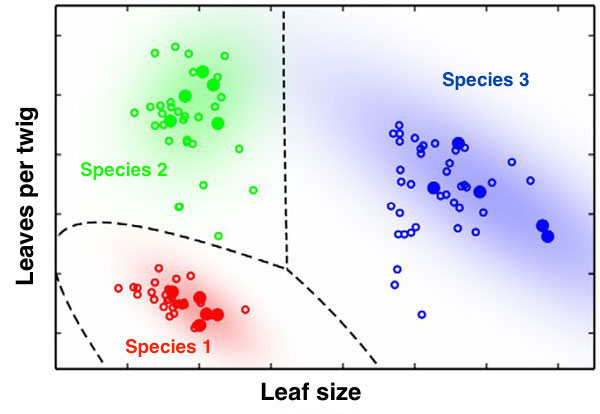
\includegraphics[width=0.6\textwidth]{images/Classification.jpg}
 
\end{figure}

\end{frame}
\subsection{Clustering}
\begin{frame}{Data Mining}{Clustering}

\begin{itemize}
\item Clustering is the process of grouping a set of data objects into multiple groups or clusters
so that objects within a cluster have high similarity, but are very dissimilar to objects in
other clusters.
\item Dissimilarities and similarities are assessed based on the attribute values describing the
objects and often involve distance measures.

\end{itemize}
\begin{figure}[H]
	\centering
	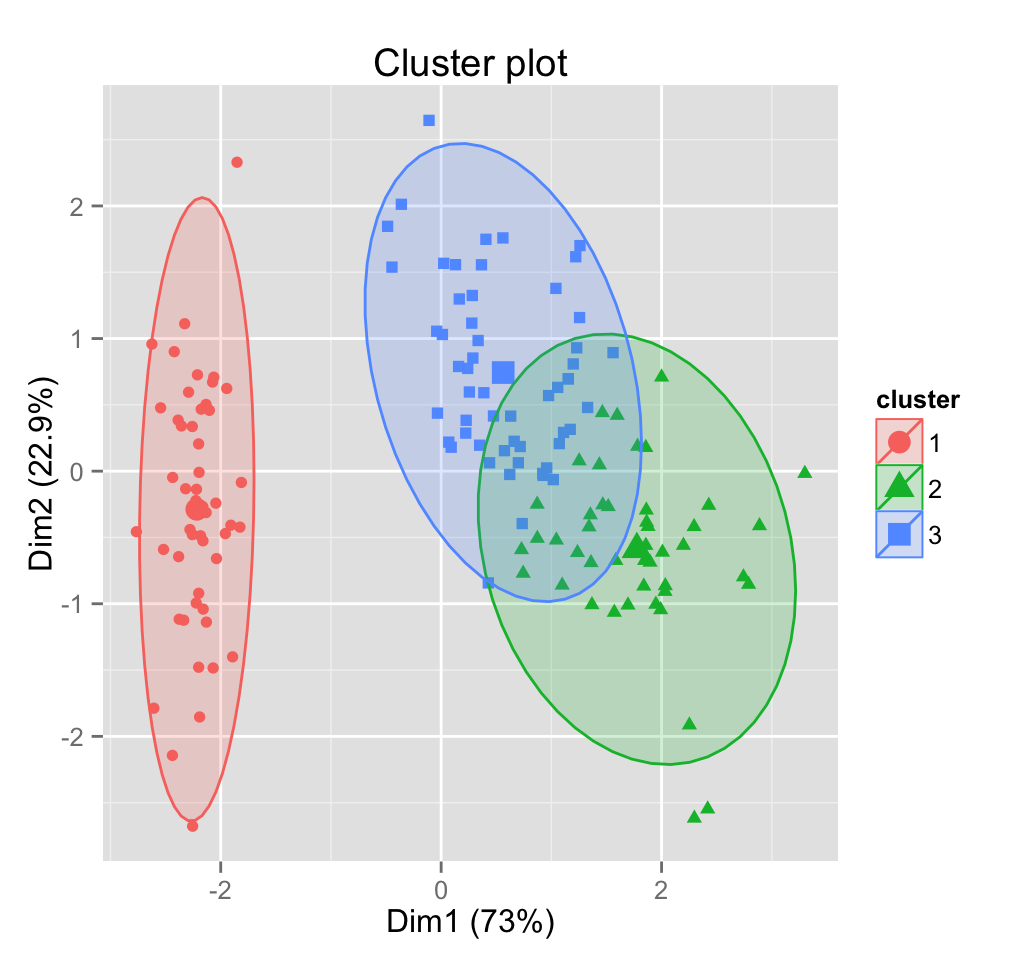
\includegraphics[width=0.5\textwidth]{images/clustering.png}

\end{figure}
\end{frame}
\subsection{Association Rule Mining}
\begin{frame}{Data Mining}{Association Rule Mining}
\begin{itemize}
\item The classical problem of associative pattern mining is defined in the context of
supermarket (items bought by customers as transactions).
\item The goal is to determine association between groups of items bought by customers.
\item The most popular model for associative pattern mining uses the frequencies of sets of
items as the quantification of the level of association.
\item The discovered set of items are referred to as large itemsets, frequent itemsets, or
frequent patterns.
\begin{figure}[H]
	\centering
	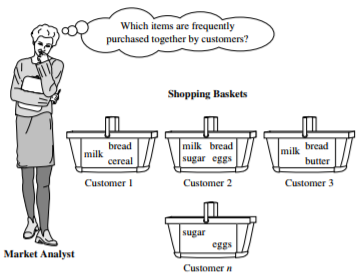
\includegraphics[width=0.4\textwidth]{images/Association.PNG}
	\label{fig:Classification}
\end{figure}
\end{itemize}
\end{frame}


\begin{frame}{Data Mining}{Association Rule Mining}
\begin{itemize}
\item Frequent itemsets can be used to generate association rules of the form
$X \rightarrow Y$\\
X and Y are set of items.
\item For example, if the supermarket owner discovers the following rule
$\{Eggs, Milk\} \rightarrow \{Yogurt\}$
\item As a conclusion, she/he can promote Yogurt to customers who often buy Eggs and Milk.
\item The frequency-based model for associative pattern mining is very popular due to its
simplicity.

\end{itemize}
\end{frame}
\section{Semantic Web Mining}

\begin{frame}{Semantic Web Mining}
\begin{itemize}
	\item Semantic web in data mining \cite{ristoski2016semantic}
	\begin{itemize}
		\item Concerned with deriving higher-level insights from data
		\item Are knowledge intensive and can often benefit from using additional knowledge from various sources
		\item Document classification, Document clustering \cite{berendt2004roadmap}
	\end{itemize}
	\item Data mining in semantic web \cite{d2010inductive}

\end{itemize}
\end{frame}

\subsection{Data mining in Semantic Web}
\begin{frame}{Semantic Web Mining}{Data mining in Semantic Web}
	Why we need it? \cite{d2010inductive}
	 \begin{itemize} 
		\item In presence of noisy/inconsistent knowledge bases, that could be highly probable in  the Web, deductive reasoning is no more applicable 
		\item inductive reasoning is grounded on the generalization of specific examples (assertions in the SW context) allowing the formulation of conclusions even when inconsistent/noisy knowledge bases are considered
		\item The main focus is on   building the terminology of an ontology while less attention has been dedicated to the enrichment/construction of the assertional part
		\item enrichment/construction of the assertional part, namely the ontology population problem results in an even more time consuming task
	 \end{itemize}
\end{frame}

\subsection{Classification}
\begin{frame}{Semantic Web Mining}{Classification}
	\begin{itemize}
		\item Ontology population task: the problem has been focused by casting it to a classification problem \cite{d2010inductive}
	 	\item Requires some assumption
	 		\begin{enumerate}
				\item Open world assumption
				\item Non-disjointness of the classes
				\item the availability of new similarity measures to exploit the expressiveness of DLs 
	 		\end{enumerate}
 		\item Nearest Neighbor (NN) and Support Vector Machine have been used in studies.
	\end{itemize}
\end{frame}
\subsection{Clustering}
\begin{frame}{Semantic Web Mining}{Clustering}
	\begin{itemize}
	\item Ontology learning task: focuses on learning ontologies (mainly terminologies) from text documents by the use of clustering methods \cite{d2010inductive}
		\begin{enumerate}
			\item Concepts are extracted from documents by the use of Natural Language Processing techniques   
			\item Concept are clustered to obtain an initial terminology 
			\item Enriched with new relationships  by means of association rules
		\end{enumerate}
	\item There are some drawbacks 
		\begin{enumerate}
			\item Semantic relations among the terms are not fully clear 
			\item Expressiveness of the adopted language is less than OWL
		\end{enumerate}
	\end{itemize}
\end{frame}

\subsection{Association Rule Mining}
\begin{frame}{Semantic Web Mining}{Association Rule Mining}
\begin{itemize}
		 
	\item Association rule mining has following applications in semantic web
		\begin{enumerate}
			\item Enriching ontology \cite{abedjan2014amending} \cite{d2012semantic}
			\item Finding new relations \cite{abedjan2013improving}
			\item Discrimination discovery \cite{luong2016classification}
			\item Building ontologies \cite{das2016semantic}
			\item Ontology alignment 
			\cite{galarraga2013mining}
			
		\end{enumerate}
\end{itemize}
\end{frame}

\section{Association Rule Mining}
\subsection{Challenges}
\begin{frame}{Association Rule Mining}{Challenges}
	There are some challenges in semantic rule mining (also in semantic web mining)  \cite{nebot2012finding}
	\begin{itemize}
		 
		\item  DM algorithms input vs ontology representation: The usual way to represent these assertions is as triples (subject, predicate, object) the identification of transactions and items is not trivial
		\item Structural heterogeneity issues: OWL is sustained by description logics (DLs), annotated data does not follow a rigid structure. That is, instances belonging to the same OWL class may have different structures
		\item Implicit data: Since DLs are defined with formal semantics, reasoning capabilities must be applied in order to handle the implicit knowledge 
	\end{itemize}
\end{frame}


\subsection{Related Works}

\begin{frame}{Association Rule Mining}{Related Works:  Improving RDF Data Through Association Rule Mining}
Improving RDF Data Through Association Rule Mining \cite{abedjan2013improving}
\begin{itemize}
	
	\item Introduce “mining configurations”, which allow us to mine RDF data sets in various ways
	\item Different configurations enable us to identify schema and value dependencies that in combination result in interesting use cases
	\item Present rule-based approaches for predicate suggestion, data enrichment, ontology improvement, and query relaxation
	\item Previous work concentrates on inductive logic programming and graph mining, or is restricted to scenarios where domain knowledge and complete ontology structures are available
\end{itemize}
\end{frame}

\begin{frame}{Association Rule Mining}{Related Works:  Improving RDF Data Through Association Rule Mining}

\begin{itemize}
\item configuration specifies one element of the SPO construct as the context of rule mining (the transaction identifiers) and another as the target of rule mining (the items and transactions)

\begin{figure} 
	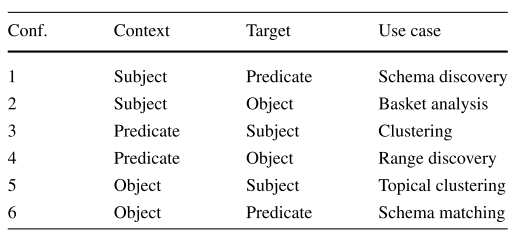
\includegraphics[width=.6\linewidth]{images/rule-config.PNG}
\end{figure}


\end{itemize}
\end{frame}

\begin{frame}{Association Rule Mining}{Related Works:  Amending RDF entities with new facts}
\begin{itemize}
\item Amending RDF entities with new facts \cite{abedjan2014amending}
\begin{enumerate}
\item Mining RDF predicates and supports manual statement creation by suggesting new predicates : reasonable hints, prevent user from using inappropriate synonyms 
\item Mining both predicates and objects, we are able to generate entirely new statements for a given data set


\end{enumerate}
\item This approach does not rely on external data sources or structural information, such as ontologies
\item  Previous work \cite{abedjan2013improving} was user-driven auto-amendment but this approach is this approach data-driven auto-amendment
\end{itemize}
\end{frame}



\begin{frame}{Association Rule Mining}{Related Works:  Amending RDF entities with new facts}
\begin{itemize}
\item Predicate suggestion
\begin{figure} 
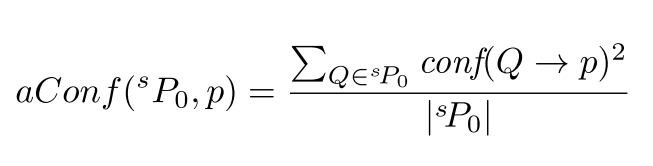
\includegraphics[width=.5\linewidth]{images/suggestion-formula.PNG}
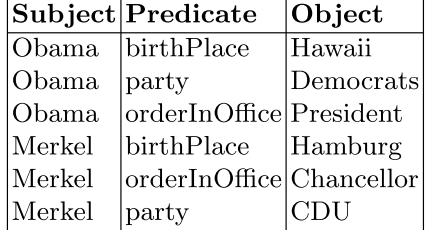
\includegraphics[width=.4\linewidth]{images/predicate-suggestion.PNG}
\end{figure}
\item For object rules $O^\prime \rightarrow o$ with high confidence (above 90 $\%$) and $O^\prime$ $ \subseteq$ O, the subjects  $S^{O^\prime} $	occurring with the objects $O^\prime$ are also likely to occur with the	object o

\end{itemize}
\end{frame}

\begin{frame}{Association Rule Mining}{Related Works:  SWARM}
An Approach for Mining Semantic Association Rules from Semantic Web Data \cite{barati2016swarm}
\begin{itemize}
\item Utilize knowledge encode in the schema-level to enrich the semantics of rules
\item introduced new support and confidence formula
\item The proposed rule quality factors (Support and confidence) consider knowledge not only in the instance-level but also schema-level ($rdf:type$ and $rdf:subClassOf$)
\item From the triples, this approach generates the following rule
\begin{figure} 
\centering
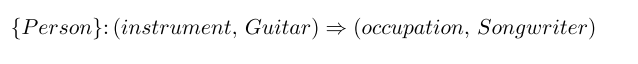
\includegraphics[width=1\linewidth]{images/swarm-example.PNG}

\end{figure}
\end{itemize}
\end{frame}

\begin{frame}{Association Rule Mining}{Related Works: Semantic Model for Web-Based Big Data}
\begin{itemize}
\item Semantic Model for Web-Based Big Data Using Ontology and Fuzzy Rule Mining \cite{das2016semantic}
\begin{itemize}
\item The use of big data and the amount of unstructured and heterogeneous information of this type is increasing.
\item  This article attempts to provide a method for structuring such data using the semantic Web.
\item This article, by combining associative rules and fuzzy logic and ontology, provides a methodology to store massive data in a structured format.
\end{itemize}
\end{itemize}
\begin{figure}[H]
	\centering
	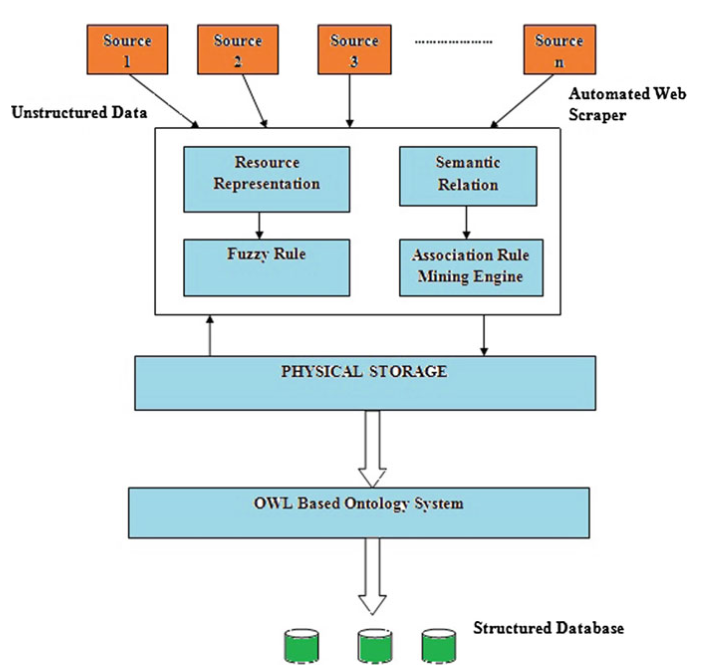
\includegraphics[width=0.43\textwidth]{images/Methodology.PNG}
	\label{fig:Methodology}
\end{figure}
\end{frame}

\begin{frame}{Association Rule Mining}{Related Works: Semantic Model for Web-Based Big Data}
\begin{itemize}
\item Mining Rules to Align Knowledge Bases \cite{galarraga2013mining}
\begin{itemize}
\item Different knowledge base can be linked together. These connections can be done at the instance level, but this is difficult at schema level, because of their inheritance structure.
\item There are many knowledge bases, each of which belongs to different companies, and many instances of them overlap, which can be connected to each other.
\item This paper assumes that the mapping is done between the instances and merges two knowledge bases.
\item It mine association rules from that Community of knowledge bases and then align them through beneath rules.
\end{itemize}
\end{itemize}

\begin{figure}[H]
	\centering
	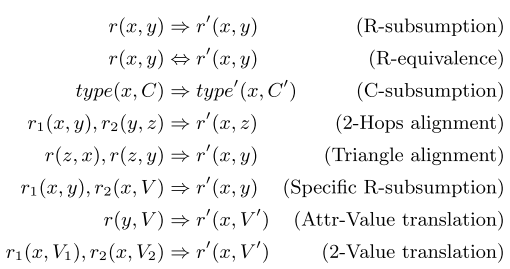
\includegraphics[width=0.5\textwidth]{images/Rosa.PNG}
	\label{fig:Rosa}
\end{figure}
\end{frame}




\begin{frame}{Association Rule Mining}{Related Works:  Semantic Knowledge Discovery}
\begin{itemize}
\item Semantic Knowledge Discovery from Heterogeneous Data Sources\cite{d2012semantic}
\begin{itemize}
\item This study combines database and ontology data and then mine association rules using Apriori.
\item A frequent itemset expresses the variables and the corresponding values that occur reasonably often together in database.
\item Now these extracted rules can help to enrich the database or ontology, or for data analysis and data completion.
\item e.g. if someone earns between 15000 and 24999 euro, he/she has a 100\% confidence of having a child and being a Child
\end{itemize}
\end{itemize}
\begin{figure}[H]
	\centering
	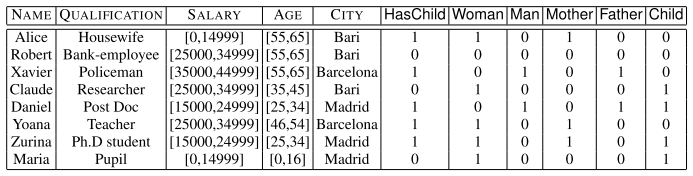
\includegraphics[width=0.8\textwidth]{images/Database.PNG}
	\label{fig:Database}
 
\end{figure}
\end{frame}


	
	



\section{References}
 \begin{frame}[allowframebreaks] {References}

\setbeamerfont{bibliography item}{size=\scriptsize}
\setbeamerfont{bibliography entry author}{size=\scriptsize}
\setbeamerfont{bibliography entry title}{size=\scriptsize}
\setbeamerfont{bibliography entry location}{size=\scriptsize}
\setbeamerfont{bibliography entry note}{size=\scriptsize}

 \bibliographystyle{plain}
\bibliography{References}
\end{frame}
%%%%%%%%%%%%%%%%

{\aauwavesbg%
\begin{frame}[plain,noframenumbering]%
  \finalpage{Thank you.}
\end{frame}}
%%%%%%%%%%%%%%%%

\end{document}
